%*******************************************************************************
%****************************** Second Chapter *********************************
%*******************************************************************************

\chapter{Introduction}

\ifpdf
    \graphicspath{{Chapter1/Figs/Raster/}{Chapter1/Figs/PDF/}{Chapter1/Figs/}}
\else
    \graphicspath{{Chapter1/Figs/Vector/}{Chapter1/Figs/}}
\fi


\subsection*{Big Data}
In the last few years Big Data generated a lot of buzz along with the launch of several successful big data products. Thanks to contribution from open source community and several giant Internet companies, the big data ecosystem has now approached a tipping point, where the basic infrastructure capabilities of supporting big data challenges are easily available. Entering the next generation of big data, so-called Big Data 2.0, two of its concentrated areas are Velocity and Applications, besides Data Quality. The cause for the former is that data is growing at an exponential rate and the ability to analyse it faster is more important than ever. For instance, sensors can generate data on millions of events per second and store all of those data and response in real-time is non trivial. The latter is helping to overcome the technical challenges of existing frameworks by making them easy to use and understand for everyone to benefit from big data.

As a result, the demand for streaming processing is increasing a lot these days. Processing big volume of data is not sufficient in the cases that infinite streaming data is arriving at high speed and users require a system to process fast and react to any incident immediately. In addition, although hardware price has plunged year over year, it’s still expensive to equip a storage which is growing terabytes every day for batch analysis.  Streaming processing engines are designed to operate high volume in real time with a scalable, high available and fault tolerant architecture.

%One of the disadvantages to users is that many big data frameworks provide a rich imperative API code only to process data stream. First, users must spend time learning API documentation properly since those APIs are fairly new to them. Therefore, the cycle time to develop products taking longer. Second, given that most big data applications are fairly simple application-wise, a block of API codes might be less optimal to use for most the popular queries. 



\subsection*{Data Streaming}
Streaming Processing is not a new concept. Indeed the similar concept, Complex Event Processing (CPE) had been proposed from the 1990s by Event Simulation Research at Stanford \citep{Luckham:2001}. Since that time, people have started generating a lot of different buzzwords around it and often reinventing ideas borrowing from other fields, but using a different vocabularies to describe the same concepts. Basically, the idea is to analyse one or multiple data streams to identify meaningful phenomena and respond to them as quickly as possible. 


According to CEP Tooling Market Survey 2014~\citep{Paul:2014}, since 1996, there has existed more than 30 companies providing Streaming Processing solutions. All the major software vendors (IBM, Oracle, Microsoft, SAP) also have good to excellent offerings in the CEP space for customers. 


However, since a massive amount of data is growing rapidly every second, Hadoop is emerging distributed processing ecosystem today. Thanks to Hadoop, people can build a large scalable distributed system on Cloud. Even though Hadoop is designed to scale system up to thousands of machines with very high degree of fault tolerance, it is optimised to run batch jobs with a huge load of computation. Because of time factor, Hadoop has limited value in online environment where fast processing is crucial. Therefore, existing CEP solutions are barely compatible with Hadoop ecosystem.  We demand a new sort of streaming framework which is able to integrate on top of Hadoop system. Apache Flink~\citep{flink} is one of these frameworks.


\subsection*{Apache Flink}

Apache Flink is an open source platform for scalable batch and stream data processing. Several innovative features make Flink standout from the Big Data world:

\textbf{Fast}: Flink exploits in-memory data streaming and integrates iterative processing deeply into the system runtime. This makes the system extremely fast for data-intensive and iterative jobs. Besides Flink also provides many more complex operations like joins, group-by, or reduce-by operations so that users can model quite complex data flows at ease.

\textbf{Reliable and Scalable}: Flink is designed to perform well when memory runs out.  Flink contains its own memory management component, serialization framework, and type inference engine.

\textbf{Easy to Use}: Flink requires few configuration parameters. And the system's bult-in optimizer takes care of finding the best way to execute the program in any enviroment.

\textbf{Compatible with Hadoop}: Flink supports all Hadoop input and output formats and data types. You can run your legacy MapReduce operators unmodified and faster on Flink. Flink can read data from HDFS and HBase, and runs on top of YARN

\begin{figure}[htbp!] 
\centering    
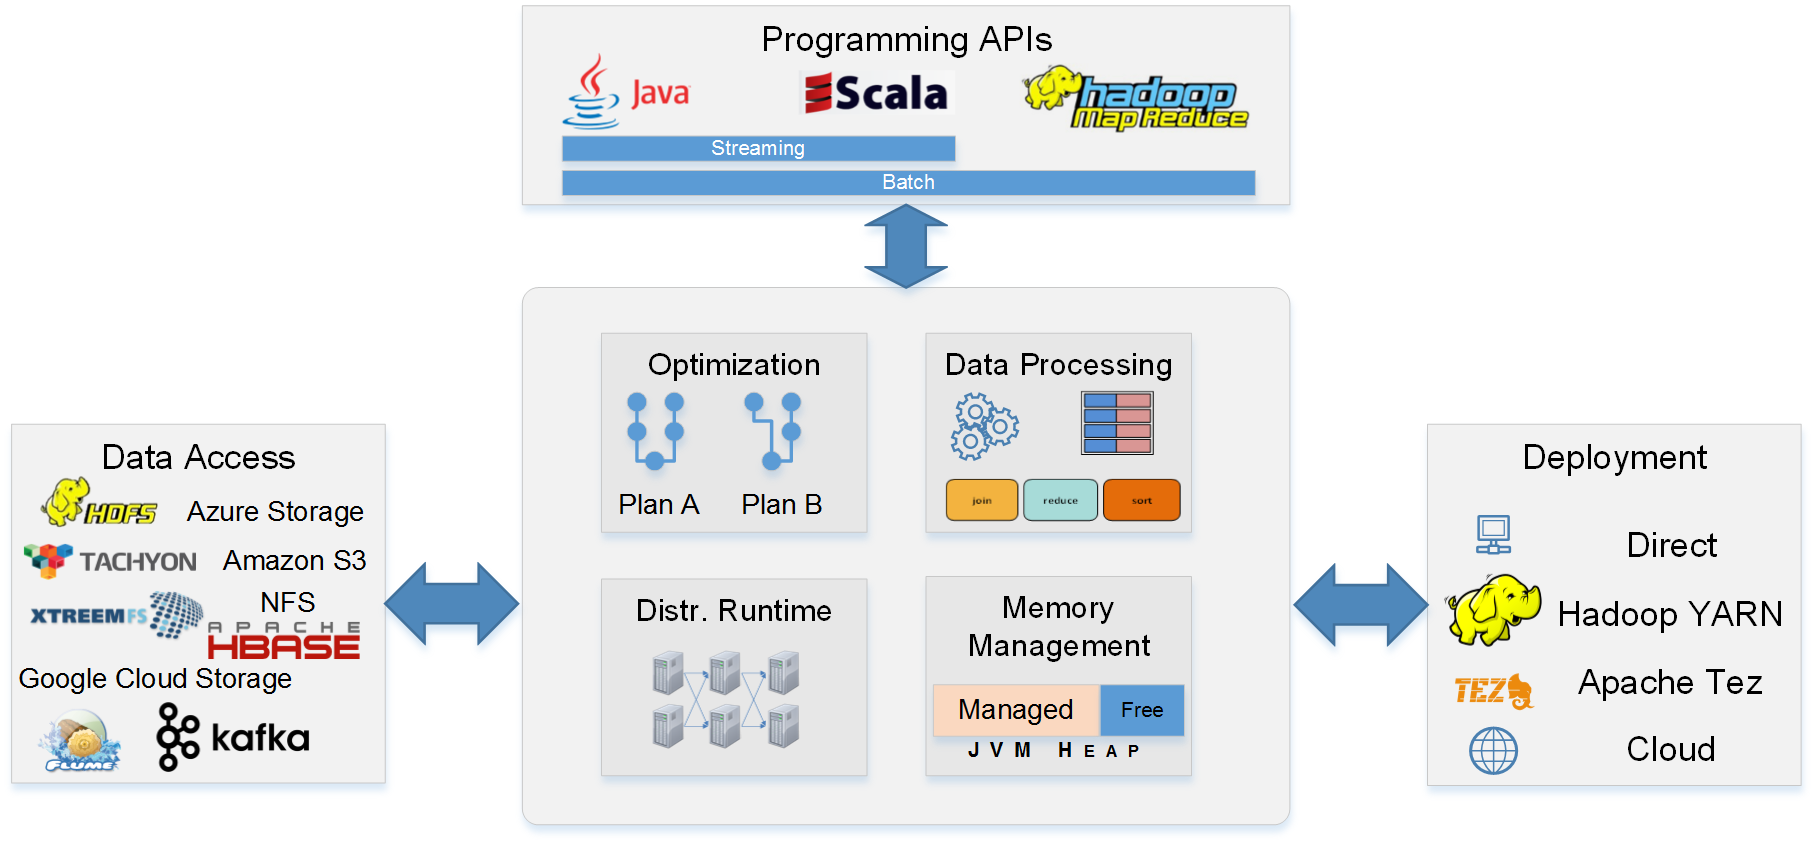
\includegraphics[width=1\textwidth]{ApacheFlink}
\caption{Apache Flink}
\label{fig:flink}
\end{figure}


Flink contains APIs in Java and Scala for analyzing data from batch and streaming data sources, as well as its own optimizer and distributed runtime with custom memory management (Figure~\ref{fig:flink})

However, similar to most of big data frameworks providing such rich APIs for imperative programing only, Flink is still struggling to gain traction from enterprise in relation of interaction UX.  First, users must spend time learning API documentation properly since those APIs are fairly new to them. Therefore, the cycle time to develop products taking longer. Second, given that most big data applications are fairly simple application-wise, a block of API codes might be less optimal to use for most the popular queries. We tackle solving the problem by building a extended version of ubiquitous SQL language on application layer of Flink. Since SQL is so popular, compact, well-design and easy to use, it is the most suitable choice to rely on for our extension. In the first step, this thesis aims to analyze streaming execution model in order to design and implement an SQL-extension (FlinkCQL - Flink Continuous Query Language) for Flink Stream Processing Engine.


\subsection*{Structure}
We present our works in 5 following chapters:
\begin{itemize}
	\item \textbf{Chapter 2:} \textit{Data Stream Model}. The chapter describes the concept of data stream and what are the differences between data stream and traditional database. 
	
	\item \textbf{Chapter 3:} \textit{The execution semantic of  Flink Stream Processing}. This part helps to understand how the streaming processing engine works under the hood.
	
	\item \textbf{Chapter 4:} \textit{FlinkCQL - Queries over Data Stream}. We fully describe the specification of FlinkCQL syntax , as well as its semantics.
	
	\item \textbf{Chapter 5:} \textit{Implementations.} An tree-based query interpreter is built to translate a input query into a Flink program written in Scala. The program then operates input data streams to produce desired outputs.
	
	\item \textbf{Chapter 6:} \textit{Conclusions}
\end{itemize}

